\documentclass[12pt,a4paper]{article}

%%%%%%%%------------------------------------------------------------------------
%%%% 日常所用宏包

%% 控制页边距
% 如果是beamer文档类, 则不用geometry
\makeatletter
\@ifclassloaded{beamer}{}{\usepackage[top=2.5cm, bottom=2.5cm, left=2.5cm, right=2.5cm]{geometry}}
\makeatother

%% 控制项目列表
\usepackage{enumerate}

%% 多栏显示
\usepackage{multicol}

%% 算法环境
\usepackage{algorithm}  
\usepackage{algorithmic} 
\usepackage{float} 

%% 网址引用
\usepackage{url}

%% 控制矩阵行距
\renewcommand\arraystretch{1.4}

%% hyperref宏包,生成可定位点击的超链接,并且会生成pdf书签
\makeatletter
\@ifclassloaded{beamer}{
\usepackage{hyperref}
}{
\usepackage[%
    pdfstartview=FitH,%
    CJKbookmarks=true,%
    bookmarks=true,%
    bookmarksnumbered=true,%
    bookmarksopen=true,%
    colorlinks=true,%
    citecolor=blue,%
    linkcolor=blue,%
    anchorcolor=green,%
    urlcolor=blue%
]{hyperref}
}
\makeatother



\makeatletter % 如果是 beamer 不需要下面两个包
\@ifclassloaded{beamer}{

}{
%% 控制标题
\usepackage{titlesec}
%% 控制目录
\usepackage{titletoc}
}
\makeatother

%% 控制表格样式
\usepackage{booktabs}

%% 控制字体大小
\usepackage{type1cm}

%% 首行缩进,用\noindent取消某段缩进
\usepackage{indentfirst}

%% 支持彩色文本、底色、文本框等
\usepackage{color,xcolor}

%% AMS LaTeX宏包: http://zzg34b.w3.c361.com/package/maths.htm#amssymb
\usepackage{amsmath,amssymb}

%%%% 基本插图方法
%% 图形宏包
\usepackage{graphicx}

%% 多个图形并排
\usepackage{subfig}

%%%% 基本插图方法结束

%%%% pgf/tikz绘图宏包设置
\usepackage{pgf,tikz}
\usetikzlibrary{shapes,automata,snakes,backgrounds,arrows}
\usetikzlibrary{mindmap}
%% 可以直接在latex文档中使用graphviz/dot语言,
%% 也可以用dot2tex工具将dot文件转换成tex文件再include进来
%% \usepackage[shell,pgf,outputdir={docgraphs/}]{dot2texi}
%%%% pgf/tikz设置结束


\makeatletter % 如果是 beamer 不需要下面两个包
\@ifclassloaded{beamer}{

}{
%%%% fancyhdr设置页眉页脚
%% 页眉页脚宏包
\usepackage{fancyhdr}
%% 页眉页脚风格
\pagestyle{plain}
}

%% 有时会出现\headheight too small的warning
\setlength{\headheight}{15pt}

%% 清空当前页眉页脚的默认设置
%\fancyhf{}
%%%% fancyhdr设置结束


\makeatletter % 对 beamer 要重新设置
\@ifclassloaded{beamer}{

}{
%%%% 设置listings宏包用来粘贴源代码
%% 方便粘贴源代码,部分代码高亮功能
\usepackage{listings}

%% 设置listings宏包的一些全局样式
%% 参考http://hi.baidu.com/shawpinlee/blog/item/9ec431cbae28e41cbe09e6e4.html
\lstset{
showstringspaces=false,              %% 设定是否显示代码之间的空格符号
numbers=left,                        %% 在左边显示行号
numberstyle=\tiny,                   %% 设定行号字体的大小
basicstyle=\footnotesize,                    %% 设定字体大小\tiny, \small, \Large等等
keywordstyle=\color{blue!70}, commentstyle=\color{red!50!green!50!blue!50},
                                     %% 关键字高亮
frame=shadowbox,                     %% 给代码加框
rulesepcolor=\color{red!20!green!20!blue!20},
escapechar=`,                        %% 中文逃逸字符,用于中英混排
xleftmargin=2em,xrightmargin=2em, aboveskip=1em,
breaklines,                          %% 这条命令可以让LaTeX自动将长的代码行换行排版
extendedchars=false                  %% 这一条命令可以解决代码跨页时,章节标题,页眉等汉字不显示的问题
}}
\makeatother
%%%% listings宏包设置结束


%%%% 附录设置
\makeatletter % 对 beamer 要重新设置
\@ifclassloaded{beamer}{

}{
\usepackage[title,titletoc,header]{appendix}
}
\makeatother
%%%% 附录设置结束


%%%% 日常宏包设置结束
%%%%%%%%------------------------------------------------------------------------


%%%%%%%%------------------------------------------------------------------------
%%%% 英文字体设置结束
%% 这里可以加入自己的英文字体设置
%%%%%%%%------------------------------------------------------------------------

%%%%%%%%------------------------------------------------------------------------
%%%% 设置常用字体字号,与MS Word相对应

%% 一号, 1.4倍行距
\newcommand{\yihao}{\fontsize{26pt}{36pt}\selectfont}
%% 二号, 1.25倍行距
\newcommand{\erhao}{\fontsize{22pt}{28pt}\selectfont}
%% 小二, 单倍行距
\newcommand{\xiaoer}{\fontsize{18pt}{18pt}\selectfont}
%% 三号, 1.5倍行距
\newcommand{\sanhao}{\fontsize{16pt}{24pt}\selectfont}
%% 小三, 1.5倍行距
\newcommand{\xiaosan}{\fontsize{15pt}{22pt}\selectfont}
%% 四号, 1.5倍行距
\newcommand{\sihao}{\fontsize{14pt}{21pt}\selectfont}
%% 半四, 1.5倍行距
\newcommand{\bansi}{\fontsize{13pt}{19.5pt}\selectfont}
%% 小四, 1.5倍行距
\newcommand{\xiaosi}{\fontsize{12pt}{18pt}\selectfont}
%% 大五, 单倍行距
\newcommand{\dawu}{\fontsize{11pt}{11pt}\selectfont}
%% 五号, 单倍行距
\newcommand{\wuhao}{\fontsize{10.5pt}{10.5pt}\selectfont}
%%%%%%%%------------------------------------------------------------------------


%% 设定段间距
\setlength{\parskip}{0.5\baselineskip}

%% 设定行距
\linespread{1}


%% 设定正文字体大小
% \renewcommand{\normalsize}{\sihao}

%制作水印
\RequirePackage{draftcopy}
\draftcopyName{XTUMESH}{100}
\draftcopySetGrey{0.90}
\draftcopyPageTransform{40 rotate}
\draftcopyPageX{350}
\draftcopyPageY{80}

%%%% 个性设置结束
%%%%%%%%------------------------------------------------------------------------


%%%%%%%%------------------------------------------------------------------------
%%%% bibtex设置

%% 设定参考文献显示风格
% 下面是几种常见的样式
% * plain: 按字母的顺序排列,比较次序为作者、年度和标题
% * unsrt: 样式同plain,只是按照引用的先后排序
% * alpha: 用作者名首字母+年份后两位作标号,以字母顺序排序
% * abbrv: 类似plain,将月份全拼改为缩写,更显紧凑
% * apalike: 美国心理学学会期刊样式, 引用样式 [Tailper and Zang, 2006]

\makeatletter
\@ifclassloaded{beamer}{
\bibliographystyle{apalike}
}{
\bibliographystyle{unsrt}
}
\makeatother


%%%% bibtex设置结束
%%%%%%%%------------------------------------------------------------------------

%%%%%%%%------------------------------------------------------------------------
%%%% xeCJK相关宏包

\usepackage{xltxtra,fontspec,xunicode}
\usepackage[slantfont, boldfont]{xeCJK} 

%% 针对中文进行断行
\XeTeXlinebreaklocale "zh"             

%% 给予TeX断行一定自由度
\XeTeXlinebreakskip = 0pt plus 1pt minus 0.1pt

%%%% xeCJK设置结束                                       
%%%%%%%%------------------------------------------------------------------------

%%%%%%%%------------------------------------------------------------------------
%%%% xeCJK字体设置

%% 设置中文标点样式,支持quanjiao、banjiao、kaiming等多种方式
\punctstyle{kaiming}                                        
                                                     
%% 设置缺省中文字体
\setCJKmainfont[BoldFont={Adobe Heiti Std}, ItalicFont={Adobe Kaiti Std}]{Adobe Song Std}   
%% 设置中文无衬线字体
\setCJKsansfont[BoldFont={Adobe Heiti Std}]{Adobe Kaiti Std}  
%% 设置等宽字体
\setCJKmonofont{Adobe Heiti Std}                            

%% 英文衬线字体
\setmainfont{DejaVu Serif}                                  
%% 英文等宽字体
\setmonofont{DejaVu Sans Mono}                              
%% 英文无衬线字体
\setsansfont{DejaVu Sans}                                   

%% 定义新字体
\setCJKfamilyfont{song}{Adobe Song Std}                     
\setCJKfamilyfont{kai}{Adobe Kaiti Std}
\setCJKfamilyfont{hei}{Adobe Heiti Std}
\setCJKfamilyfont{fangsong}{Adobe Fangsong Std}
\setCJKfamilyfont{lisu}{LiSu}
\setCJKfamilyfont{youyuan}{YouYuan}

%% 自定义宋体
\newcommand{\song}{\CJKfamily{song}}                       
%% 自定义楷体
\newcommand{\kai}{\CJKfamily{kai}}                         
%% 自定义黑体
\newcommand{\hei}{\CJKfamily{hei}}                         
%% 自定义仿宋体
\newcommand{\fangsong}{\CJKfamily{fangsong}}               
%% 自定义隶书
\newcommand{\lisu}{\CJKfamily{lisu}}                       
%% 自定义幼圆
\newcommand{\youyuan}{\CJKfamily{youyuan}}                 

%%%% xeCJK字体设置结束
%%%%%%%%------------------------------------------------------------------------

%%%%%%%%------------------------------------------------------------------------
%%%% 一些关于中文文档的重定义
\newcommand{\chntoday}{\number\year\,年\,\number\month\,月\,\number\day\,日}
%% 数学公式定理的重定义

%% 中文破折号,据说来自清华模板
\newcommand{\pozhehao}{\kern0.3ex\rule[0.8ex]{2em}{0.1ex}\kern0.3ex}

\newtheorem{example}{例}                                   
\newtheorem{theorem}{定理}[section]                         
\newtheorem{definition}{定义}
\newtheorem{axiom}{公理}
\newtheorem{property}{性质}
\newtheorem{proposition}{命题}
\newtheorem{lemma}{引理}
\newtheorem{corollary}{推论}
\newtheorem{remark}{注解}
\newtheorem{condition}{条件}
\newtheorem{conclusion}{结论}
\newtheorem{assumption}{假设}

\makeatletter %
\@ifclassloaded{beamer}{

}{
%% 章节等名称重定义
\renewcommand{\contentsname}{目录}     
\renewcommand{\indexname}{索引}
\renewcommand{\listfigurename}{插图目录}
\renewcommand{\listtablename}{表格目录}
\renewcommand{\appendixname}{附录}
\renewcommand{\appendixpagename}{附录}
\renewcommand{\appendixtocname}{附录}
%% 设置chapter、section与subsection的格式
\titleformat{\chapter}{\centering\huge}{第\thechapter{}章}{1em}{\textbf}
\titleformat{\section}{\centering\sihao}{\thesection}{1em}{\textbf}
\titleformat{\subsection}{\xiaosi}{\thesubsection}{1em}{\textbf}
\titleformat{\subsubsection}{\xiaosi}{\thesubsubsection}{1em}{\textbf}

\@ifclassloaded{book}{

}{
\renewcommand{\abstractname}{摘要}
}
}
\makeatother

\renewcommand{\figurename}{图}
\renewcommand{\tablename}{表}

\makeatletter
\@ifclassloaded{book}{
\renewcommand{\bibname}{参考文献}
}{
\renewcommand{\refname}{参考文献} 
}
\makeatother

\floatname{algorithm}{算法}
\renewcommand{\algorithmicrequire}{\textbf{输入:}}
\renewcommand{\algorithmicensure}{\textbf{输出:}}

%%%% 中文重定义结束
%%%%%%%%------------------------------------------------------------------------

\numberwithin{equation}{section}
\renewcommand {\thetable} {\thesection{}.\arabic{table}}
\renewcommand {\thefigure} {\thesection{}.\arabic{figure}}
\title{并行计算}
\author{}
\date{\chntoday}
\begin{document}
\maketitle

\section{Linux操作系统与程序开发环境}
本章介绍 Linux 的安装和基本使用,以及在Linux 操作系统上进行程序开发的简单知识。
\subsection{Linux安装与使用入门}
\subsubsection{Linux 系统的安装}
Linux 系统默认的文件系统格式是 ext2 ,或它的后继 ext3等 。和其他操作系统一样, Linux 的文件系统采用的也是树形结构,树的根就是 根目录(root directory) ,用一个正斜杠 “/” 表示,树的叶子是文件,中间结点则是目录。要注意的是, Linux 的路径名中用正斜杠“/” 分隔目录名,而 Windows 中用的则是反斜杠 “$\setminus$” 。 Linux 系统的
根目录下通常有下面一些子目录:

$\bullet$~/usr :其中安装着主要的系统文件和软件;

$\bullet$~/home :普通用户的家目录所在的位置,可以选择将它放在一个不同的硬盘分区上,这样在重新安装系统时可以保留用户的文件;

$\bullet$~/etc :系统配置文件;

$\bullet$~/dev :设备文件,主要用于驱动各类硬件;

$\bullet$~/proc :该目录中的内容不是硬盘上的普通文件,而是 Linux 内核的一些接口,通过它可以在运行时获取、改变系统内核的许多参数;

$\bullet$~/mnt :外挂设备的挂接点;

$\bullet$~/root :超级用户的家目录;

$\bullet$~/sbin :包含一些主要供超级用户用的可执行程序;

$\bullet$~/bin :一些最常用的可执行程序;

$\bullet$~/boot 和 /initrd :系统启动用的文件;

$\bullet$~/lib :库文件;

$\bullet$~/tmp :用于创建临时文件或目录;

$\bullet$~其他目录: /opt , /misc , /var :这些目录普通用户基本上不用;需要指出的是系统日志文件在目录 /var/log 下面。

$\bullet$~bin 和 sbin :包含可执行文件,其中 sbin 中的文件主要是系统管理员用的;

$\bullet$~lib :主要的库文件的位置,它常常是最占空间的;

$\bullet$~include :头文件的位置,编写程序时需要包含的头文件大都在这个目录中;

$\bullet$~src :内核和软件的源代码的位置;

$\bullet$~local :这是安装一些外来软件的地方,有些软件也可能选择安装在 /opt ;

$\bullet$~X11R6 :和 X 有关的文件,包括可执行命令、头文件、库文件等等。 X 是 Linux/UNIX 的图形界面软件,图形用户界面的软件通常都在该目录中;

$\bullet$~share/man 和 share/doc :帮助文件所在的位置;

\subsubsection{基本使用与管理}
启动进入 Linux 系统后,首先看到的是一个登录界面,输入创建的用户名和密码。Linux 最基本的系统管理工作包括系统配置、用户帐户管理、安装和卸载软件包。为了进行系统管理工作,首先需要获得管理员的身份。普通用户可以用命令 su 转换成为超级用户,为此,只需在shell 提示符前输入命令:
\begin{figure}[H]
\centering
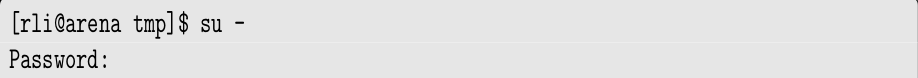
\includegraphics[scale=0.6]{./figures/21.png}
%%\caption{}
\end{figure}

\begin{figure}[H]
\centering

\includegraphics[scale=0.6]{./figures/22.png}
%%\caption{}
\end{figure}
在 su 命令后面加上可选项 “-” 的主要作用是为了得到超级用户的路径,以便直接使用 /sbin 和 /usr/sbin 中的命令。

\textbf{1.账号管理}

Linux 系统最重要的配置文件之一是 /etc/passwd ,它记载着系
统中所有用户的信息。在传统的 UNIX 系统中,该文件存储用户的
用户名、用户号、密码等信息。现代系统中出于安全考虑,把用户口
令单独存储在另外一个文件 /etc/shadow 中,所以 /etc/passwd 中
实际上并没有存储密码。Linux 中添加新用户的命令为 useradd ,它的简单语法为
\begin{figure}[H]
\centering
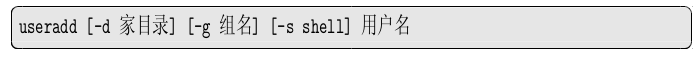
\includegraphics[scale=0.6]{./figures/23.png}
%%\caption{}
\end{figure}
家目录指定新用户的家目录 ( 默认值为 /home/ 用户名 ) ,组名指定新用户所属的用户组 ( 稍后解释 ) , shell 指定用户的默认shell ,即用户登录时自动获得的 shell ( 默认值为 /bin/bash) 。例如,
下面的命令
\begin{figure}[H]
\centering
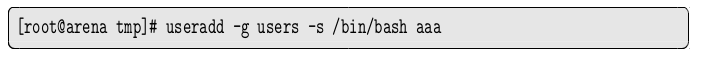
\includegraphics[scale=0.6]{./figures/24.png}
%%\caption{}
\end{figure}
添加一个名为 aaa 的新用户,该用户属于用户组 users , shell 为
/bin/bash 。

删除一个用户的命令为
\begin{figure}[H]
\centering
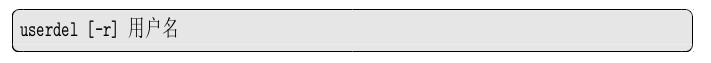
\includegraphics[scale=0.6]{./figures/25.png}
%%\caption{}
\end{figure}
修改用户密码的命令是 passwd ,语法如下:
\begin{figure}[H]
\centering
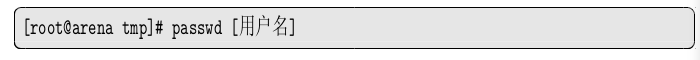
\includegraphics[scale=0.6]{./figures/26.png}
%%\caption{}
\end{figure}
超级用户可以修改任何用户的密码,普通用户只能修改自己的密码。

命令 usermod 可用来修改一个帐号的属性。它的命令行参数和
useradd 基本一样。如:
\begin{figure}[H]
\centering
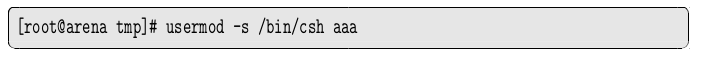
\includegraphics[scale=0.6]{./figures/27.png}
%%\caption{}
\end{figure}
会将用户 aaa 的默认 shell 改成 C shell (/bin/csh) 。

为了便于管理, Linux 系统中的用户被分成一个个的用户组,每个用户可以同时属于多个用户组, /etc/passwd 中给出的用户组是该用户的默认用户组。

系统有时候会给出一个提示,说用户的密码已经过期了。密码的期限可以通过
命令 chage 来查询或设置,它的语法为:
\begin{figure}[H]
\centering
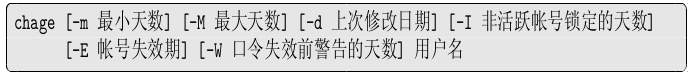
\includegraphics[scale=0.6]{./figures/28.png}
%%\caption{}
\end{figure}
\textbf{2.软件包管理}

Linux下常见的压缩包格式有5种:zip ~tar.gz ~tar.bz2 ~tar.xz ~tar.Z

filename.zip的解压:
\begin{figure}[H]
\centering

\includegraphics[scale=0.6]{./figures/284.png}
%%\caption{}
\end{figure}
filename.tar.gz的解压:
\begin{figure}[H]
\centering
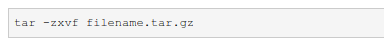
\includegraphics[scale=0.6]{./figures/285.png}
%%\caption{}
\end{figure}

\begin{figure}[H]
\centering
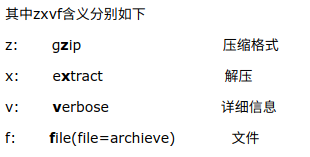
\includegraphics[scale=0.6]{./figures/286.png}
%%\caption{}
\end{figure}

filename.tar.bz2的解压:
\begin{figure}[H]
\centering
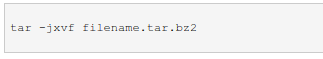
\includegraphics[scale=0.6]{./figures/287.png}
%%\caption{}
\end{figure}
其它选项和tar.gz解压含义相同

filename.tar.xz的解压: 
\begin{figure}[H]
\centering
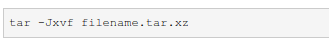
\includegraphics[scale=0.6]{./figures/288.png}
%%\caption{}
\end{figure}
filename.tar.Z的解压: 
\begin{figure}[H]
\centering
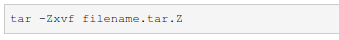
\includegraphics[scale=0.6]{./figures/289.png}
%%\caption{}
\end{figure}


在 Linux 下,人们比较喜欢使用 gzip 或者 bzip2 进行文件的压缩,这两种压缩文件的扩展名分别是 “.gz” 和 “.bz2” 。同时,在压缩以前,一般会使用tar 工具对源程序的整个目录进行归档,这类归档文件的扩展名为“.tar” 。这样,一个软件包源码的整个名字通常是 “xxxx.tar.gz”或者 “xxxx.tar.bz2” 的形式,有时候也可能会将 “.tar.gz” 合并为 “.tgz” 。对于这样的软件包,其编译、安装步骤大都是类似的。以 Kile 为例,它是 Linux 下编写 TEX 文档的一个前端软件 ( 事实上, Kile 已经是 Fedora Core 中的标准包,可以在安装 Linux 系统时直接选择或用 yum 安装 ) 。假设源码文件名为 kile-1.5.tar.gz ,放在临时目录 /tmp 下。\\
$\bullet$~ 解开源码包:
\begin{figure}[H]
\centering
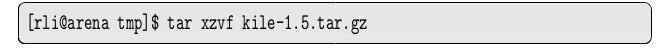
\includegraphics[scale=0.6]{./figures/266.png}
%%\caption{}
\end{figure}
“x” 表示展开档案, “v” 表示打印出操作时的信息, “f” 表示对紧随其后的文件进行操作, “z”表示是 gzip 格式的压缩文件 ( 如果是 bzip2 的压缩文件则需用 “j”) 。下面的命令也可以做到同样的事情,它通过稍后要介绍的管道进行操作:
\begin{figure}[H]
\centering
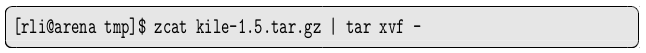
\includegraphics[scale=0.6]{./figures/210.png}
%%\caption{}
\end{figure}
软件包解开后,会在当前目录下产生一个子目录 kile-1.5 。进入该子目录,可以看到很多文件,包括: configure , configure.in ,
configure.ac , Makefile.in , Makefile.am 等等,它们用于 Kile软件的配置与编译。目录下还有帮助用户了解和安装该软件的一些文档,比如 README , INSTALL , NEWS 等,它们都是普通的文本文件,其含义一目了然,编译、安装前最好先仔细阅读这些文档。\\
$\bullet$~运行 configure 脚本进行系统检测,产生 Makefile 文件:
\begin{figure}[H]
\centering
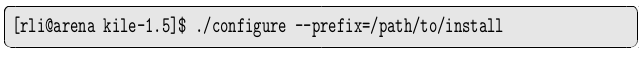
\includegraphics[scale=0.6]{./figures/211.png}
%%\caption{}
\end{figure}
其中 --prefix 选项指定软件的安装路径,默认的安装路径一般是 /usr/local 。 configure 运行完毕后,会产生一个新的Makefile 文件。\\
$\bullet$~编译软件:
\begin{figure}[H]
\centering

\includegraphics[scale=0.6]{./figures/212.png}
%%\caption{}
\end{figure}
make 是 Linux 系统中的命令,它根据当前目录下的 Makefile 文
件完成复杂的编译和链接软件包的工作。\\
$\bullet$~安装软件:
\begin{figure}[H]
\centering

\includegraphics[scale=0.6]{./figures/213.png}
%%\caption{}
\end{figure}
要注意的是,运行安装命令时要求对安装目录有写的权限,必要时需先用 su 命令转换成超级用户再执行上面的命令。\\
$\bullet$~卸载软件包:某些软件,如这里的 Kile ,在 Makefile 中提供了
卸载功能,可用下面的命令卸载安装的软件
\begin{figure}[H]
\centering
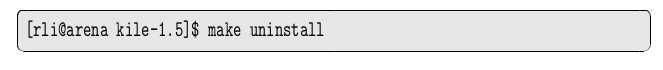
\includegraphics[scale=0.6]{./figures/214.png}
%%\caption{}
\end{figure}


\subsection{Linux基本命令和概念}
\subsubsection{一些基本命令}
下面介绍 Linux 系统的一些基本命令。

\textbf{1.}pwd~该命令显示当前工作目录。

\textbf{2.}cd~改变当前目录。cd~-回到上一次所在的目录。cd~~表示用户的家目录。cd~..表示当前目录的上一级目录。

\textbf{3.}ls列出当前目录下的文件和子目录名。ls
 命令后面指定要列出的文件或目录名。ls~-l列出当前目录下的文件和目录的细节信息。
\begin{figure}[H]
\centering
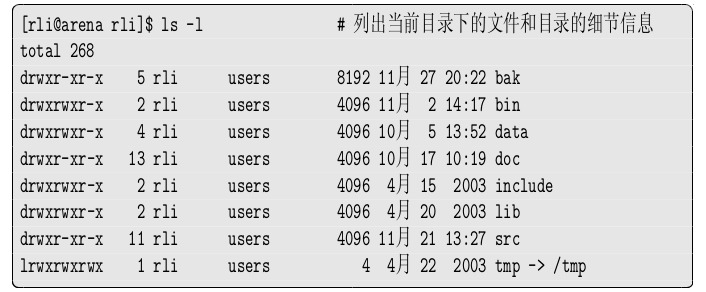
\includegraphics[scale=0.6]{./figures/215.png}
%%\caption{}
\end{figure}
上面的输出中,第一列的第一个字符给出文件的类型,这里,除了 tmp 是 “l” 以外,其余都是 “d” 。 d表示目录,而 l 表示符号链接。除了 d 和 l 外,文件类型还可以是- 、 s 、 b 、 c 和 p ,分别表示普通文件、具有 SUID 属性的文件、块设备、字符设备和管道。

Linux 是一个多用户的操作系统,系统中的每个文件都有属主(owner) ,即拥有该文件的用户。大部分系统文件的属主是超级用户,普通用户无权修改它们。每个文件除了有属主以外,还有一个用户组的属性。默认情况下,文件的组就是属主的默认组。这样,对于一个文件来说,系统上的所有用户被分成三类:第一类是该文件的属主,第二类是该文件的用户组中的用户,第三类是所有其他用户。在上面的输出中,第三列是属主 (rli) ,第四列是文件的用户组 (users) 。对一个文件的访问权限描述,也相应分成三个部分,在上面的输出中,第一列除第一个字符外的其余 9 个字符用于描述不同用户对文
件的访问权限,它们每三个字符构成一组,共三组,分别表示属主、用户组成员和其他用户对该文件的访问权限。每组三个字符依次是r (read, 表示读的权限 ) 、 w (write, 表示写的权限 ) 和 x (execute, 表示执行权限 ) ,如果具有该权限,则显示相应的字符,如果不具有该权限,则显示一个短横线 - 。比如上面输出行,
\begin{figure}[H]
\centering
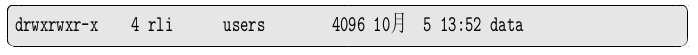
\includegraphics[scale=0.6]{./figures/216.png}
%%\caption{}
\end{figure}
表示对于目录 data ,用户 rli 有读、写和执行权限, users 组中的用户有读、写和执行权限,而其他用户只有读和执行权限,没有写权限。

\textbf{4.}echo显示命令行参数。该命令将命令行参数原封不动地显示出来。
如:
\begin{figure}[H]
\centering
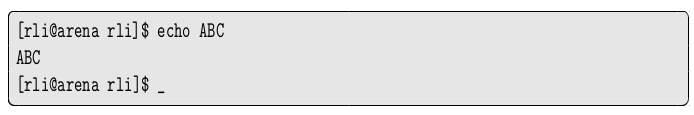
\includegraphics[scale=0.6]{./figures/217.png}
%%\caption{}
\end{figure}

\textbf{5.}file确定一个文件大致的类型与性质。
\begin{figure}[H]
\centering
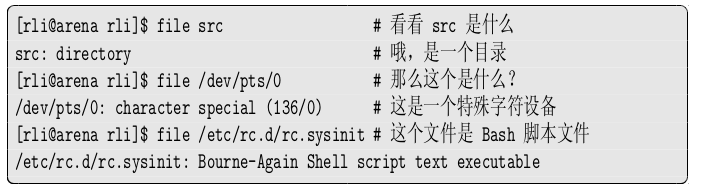
\includegraphics[scale=0.6]{./figures/218.png}
%%\caption{}
\end{figure}

\textbf{6.}man获取在线帮助。当对任何一条命令、函数、甚至关键词有疑问的时候,可以试试用 man 命令加上相应命令、函数的名称或关键词,看是否有相关的帮助信息。如
\begin{figure}[H]
\centering
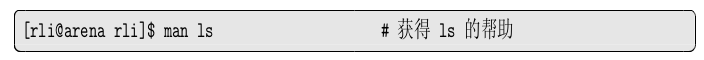
\includegraphics[scale=0.6]{./figures/219.png}
%%\caption{}
\end{figure}

\begin{figure}[H]
\centering
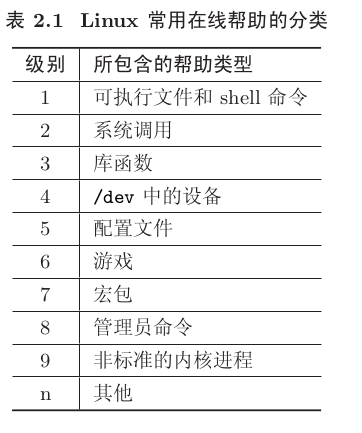
\includegraphics[scale=0.6]{./figures/220.png}
%%\caption{}
\end{figure}
例如,类别 “n” 、 “1” 和 “3” 中均有关于 “read” 的帮助信息,可以用 “man -a read” 将所有关于 read 的帮助信息找出来。

Linux 系统中除了传统的 man 格式的在线帮助之外,还有 info格式的帮助文档。 info 格式的帮助文档通常比 man 更详尽。

\textbf{7.}mkdir创建一个新目录

\textbf{8.}rm删除文件或目录x。
rm 命令的后面加了 -rf 参数,这是一种危险的使用方式。参数 “-r” 表示按照目录树递归操作, “-f” 表示不做任何提示强制删除目录下的任何文件及子目录。

\textbf{9.}cp拷贝目录或文件。它可以为一个文件建立一份新的拷贝,或者将一个或者多个文件拷贝到一个目标目录中。如果希望整个拷贝一个目录的话,可以使用 -R 、 -r 或 -a 选项。

\textbf{10.}mv移动目录或者文件。它将文件或者目录移动成为一个新的文件
或者目录,或移动到另外一个目录中。

\textbf{11.}ln为文件或目录建立链接 (link) 。Linux 系统中,一个文件或目录
的链接对应于 Windows 中的“快捷方式”,本质上相当于一个文件或目录具有多个名字。链接分硬链接和软链接 ( 也叫符号链接 ) 两种。合理使用链接往往可以方便许多系统及文件的管理工作。默认情况下, ln 命令创建硬链接。如果希望创建符号链接,则应该加上“-s” 选项。一个文件的硬链接必须与原来的文件位于同一文件系统内 ( 硬盘的同一个分区 ) ,而符号链接则无此限制。下面是创建一个目录的符号链接的例子:
\begin{figure}[H]
\centering
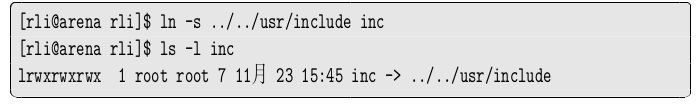
\includegraphics[scale=0.6]{./figures/221.png}
%%\caption{}
\end{figure}
注意,如果一个符号链接的对象包含的是相对路径 ( 即路径名不是
以 “/” 开头 ) ,则该对象的位置是相对于符号链接所在的目录而言
的。例如在上例中,假设当前目录是 /home/rli ,则 inc 实际所指的对象为 /home/rli/../../usr/include ,即 /usr/include 。

\textbf{12.}touch改变文件的最后修改时间。该命令也常被用来创建一个新的空文件。

\textbf{13.}cat , more , less , lv , head , tail查看文件内容。cat将输入文件的内容连接起来输出到标准输出; more 将输入文件分屏交互地显示出来; less 是对 more 功能的增强; head 显示输入文件的头十行或指定数目的行; tail 显示输入文件的最后十行或指定数目的行。这些命令支持一个或多个输入文件名做为参数。这些命令支持一个或多个输入文件名做为参数。当不给出输入文件名时,它们会从标准输入,默认情况下是用户的键盘,读入
内容,这种情况下需要用 Ctrl-D 来结束输入:
\begin{figure}[H]
\centering
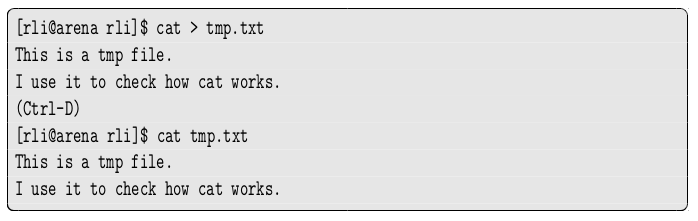
\includegraphics[scale=0.6]{./figures/222.png}
%%\caption{}
\end{figure}
上面第一个命令中使用了一个 “>” 符号,这叫做重定向,它将本来应该输出到屏幕的内容转到了文件 “tmp.txt” 中。

\textbf{14.}chmod , chgrp , chown修改文件属性。 chmod 修改文件的权限位, chgrp 修改文件所属的组, chown 则修改文件的属主。下面是 chmod 命令的例子:
\begin{figure}[H]
\centering
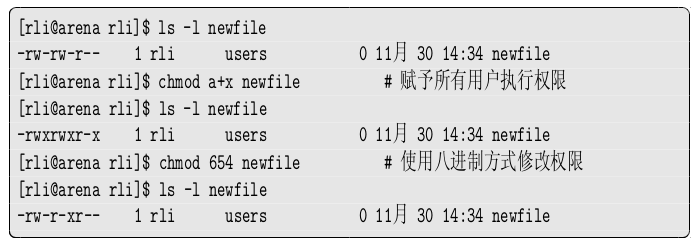
\includegraphics[scale=0.6]{./figures/223.png}
%%\caption{}
\end{figure}
chmod 命令修改文件访问权限时可以用文本或八进制两种方式来描述。使用文本描述方式时,其语法为 [ugoa][+-][rwx] ,其中第一部分表示修改哪部分用户的权限,字母 “u” 、 “g” 、 “o” 和 “a” 分别表示属主、用户组、其他用户和所有用户,第二部分表示增加 (+) 还是去除 (-) 相应的权限,而第三部分则表示是读 (r) 、写 (w) 还是执行权限 (x) 。比如 g+w 表示加上组中用户的写权限, o-x 表示去除其他用户的执行权限。如果只想增加或去除目录的执行权限 ( 表示是否允许进入 ) ,但不希望改变普通文件的执行权限,可以用大写的 “X” 。例如, “chmod a+X *” 会将当前目录中的所有子目录加上执行权限,但不改变普通文件的执行权限。

\textbf{15.}ps , kill , nice , renice , top查看和管理进程。直接使用 ps 命令可以看到现在正在运行的进程的信息;使用 kill 可以向某个进程发一个信号,通常用于改变进程的运行状态或杀死进程;使用 nice 和 renice 可以调整进程的优先级别,从而使得机器能够集中精力于更重要的进程; top 则是一个交互式的查看系统状况的工具。请看下面的例子:
\begin{figure}[H]
\centering
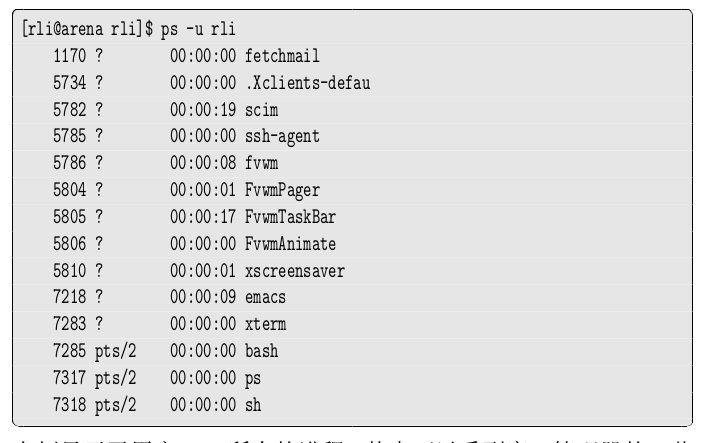
\includegraphics[scale=0.6]{./figures/224.png}
%%\caption{}
\end{figure}
上例显示了用户 rli 所有的进程。其中可以看到窗口管理器的一些进程,该用户在用 fetchmail 检查邮件,用 Emacs 编辑器进行编辑( 事实上编辑的正是本章的排版源文件 ) ,并且还启动了一个模拟终端 xterm 来运行命令 ps -u rli 。下面用 kill 来杀掉邮件检查程序fetchmail :
\begin{figure}[H]
\centering
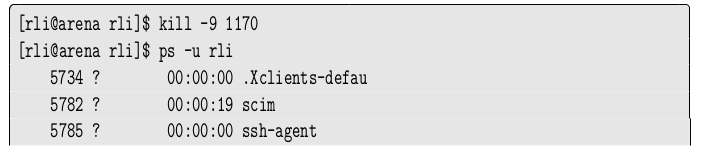
\includegraphics[scale=0.6]{./figures/225.png}
%%\caption{}
\end{figure}
命令 kill 向指定进程发送一个信号(signal) ,上例中的信号是 “9”(KILL) ,表示强制进程终止。在指定信号时,既可用信号值,如 “-9” ,“-15” 等,也可用信号的名称,如 “-KILL” 、 “-TERM” 等。当不指定信号时,默认信号为 TERM ,该信号通常终止进程的运行。下表列出了不同信号的意义。 信号可以是系统产生的,例如当发生某种异常 ( 常见的有浮点溢出、非法内存访问等 ) 或事件时,也可以由一个进程发送给另一个进程。大部分信号能够被进程捕获,进程可以自行决定如何处理这些信号。但是 9 (KILL) 是不能被捕获的,进程会立即终止。因此,除非有必要,通常应该用 “kill -TERM” 来杀死进程,以便进程在退出前完成一些必要的清理和善后的工作。
\begin{figure}[H]
\centering
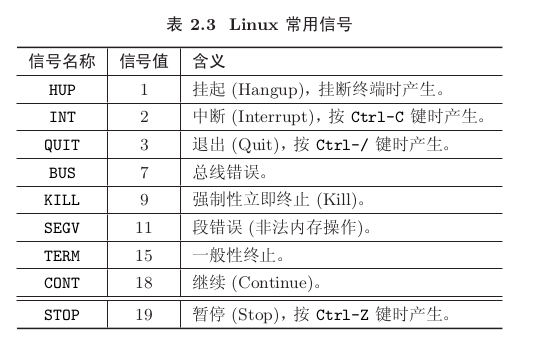
\includegraphics[scale=0.6]{./figures/269.png}
%%\caption{}
\end{figure}
nice 命令用于在启动进程时指定它的优先级别。普通用户只能降低进程的优先级别 ( 这是命令名 nice 的含义 ),而系统管理员可以调高进程的优先级。其语法为 “nice -n 调整值 [ 命令 [ 参数 ]]” ,所启动的进程会按照调整后的优先级运行。如果希望改变一个正在运行的进程的优先级,则需要用 renice 命令。

top 用于交互地监视系统的状态。运行命令时,屏幕就会成为一个字符界面的窗口,在中间分列显示系统各方面的情况,同时还可以进行一些交互操作。

\textbf{16.}\& , nohup在后台运行程序。命令后面加上一个 “\&”可以把它放到后台去运行。如果希望在后台程序运行的同时关闭终端,可以用 nohup 命令来运行程序,避免从系统退出时程序被 HUP 信号杀掉,用 nohup 运行的命令会自动将它的输出定向到文件 nohup.out 中。

\textbf{17.}fg , bg , jobs控制前台或者后台程序的运行。 fg 命令将一个后台运行的进程转到前台运行, bg 则是使得一个进程在后台运行。Ctrl+Z挂起当前任务。

命令 jobs 显示出当前 shell 中的所有作业及状态 (“Running” 、“Stopped” 等 ) 。所显示的作业中带有 “+” 号者为 当前作业。
\begin{figure}[H]
\centering
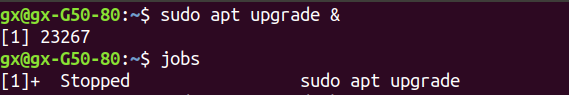
\includegraphics[scale=0.6]{./figures/291.png}
%%\caption{}
\end{figure}
\textbf{18.}find , locate搜索文件。 find 命令在指定目录中查找文件:
\begin{figure}[H]
\centering
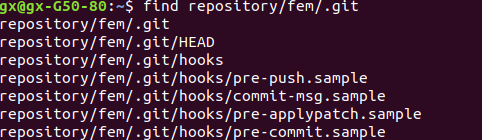
\includegraphics[scale=0.6]{./figures/267.png}
%%\caption{}
\end{figure}
locate命令其实是“find -name”的另一种写法,但是要比后者快得多,原因在于它不搜索具体目录,而是搜索一个数据库(/var/lib/locatedb),这个数据库中含有本地所有文件信息。Linux系统自动创建这个数据库,并且每天自动更新一次,所以使用locate命令查不到最新变动过的文件。为了避免这种情况,可以在使用locate之前,先使用updatedb命令,手动更新数据库。locate命令的使用实例:
\begin{figure}[H]
\centering
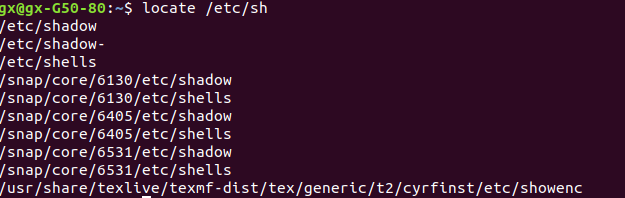
\includegraphics[scale=0.7]{./figures/292.png}
%%\caption{}
\end{figure}
whereis可以查看文件的位置,例如
\begin{figure}[H]
\centering
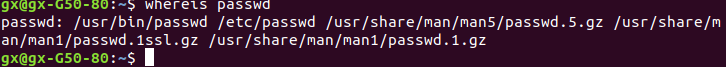
\includegraphics[scale=0.7]{./figures/293.png}
%%\caption{}
\end{figure}

\textbf{19.}grep寻找文本中的特定信息。例如,如果想在名为 ftp\_log 的日志文件中找到有哪些是来自于北京大学 (IP 地址为 162105.x.x 形式 )
的服务请求,可以使用下面的命令:
\begin{figure}[H]
\centering

\includegraphics[scale=0.6]{./figures/228.png}
%%\caption{}
\end{figure}
除 grep 外,还有 egrep 、 fgrep 和 zgrep 等命令,它们共同构成了 grep 命令家族。这些命令用正则表达式描述查找的字符串。

\textbf{20.}cut分列处理文本。通过指定分隔符号来将句子分列,然后将指定的列提取出来。
\begin{figure}[H]
\centering
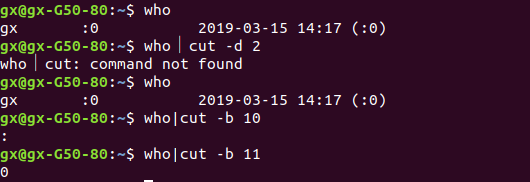
\includegraphics[scale=0.6]{./figures/229.png}
%%\caption{}
\end{figure}

\textbf{21.}tr对文本中的字符进行替换。该命令将标准输入流中的字符进行
一些简单的替换、缩并或者是删除操作。用下面的命令可以将文件中的 “\$$\hat{}~$M”
去掉:
\begin{figure}[H]
\centering
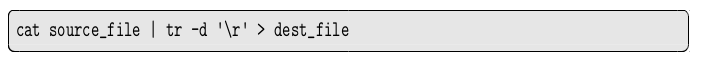
\includegraphics[scale=0.6]{./figures/268.png}
%%\caption{}
\end{figure}
该例中,选项 “-d” 表示删除输入文本中的指定字符, “$\setminus$ r” 代表字
符 “\$ $\hat{}~$M” (ASCII 字符 13) 。

\textbf{22.}who , whoami , id , w,命令 who 和 w 显示出当前登录的所有用户的信息, whoami 和id 则显示出当前用户的信息。

\textbf{23.}mount , umount , df这些命令分别用来挂载、卸载文件系统和显示当前挂载的文件系统。


\textbf{24.}bc任意精度计算器。下面是使用 bc 的一些例子:
\begin{figure}[H]
\centering
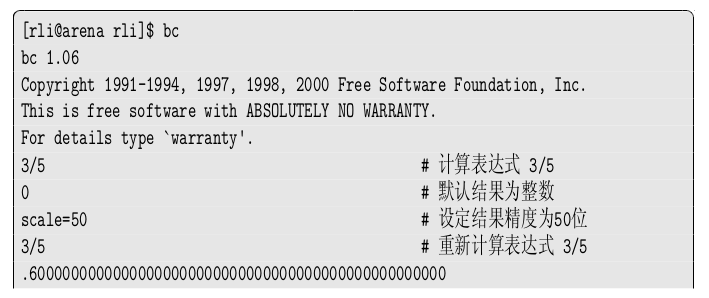
\includegraphics[scale=0.6]{./figures/230.png}
%%\caption{}
\end{figure}

\subsubsection{Shell}
这里主要介绍 Bash ,因为Linux 的许多发行版将 Bash 作为默认的 shell 。

\textbf{1.自动补全}

当在 shell 中输入命令时,只要输入命令名、目录或文件的开头几个字符,然后按 Tab 键, Bash 便会自动将名称补全。

\textbf{2.历史记录}

用 history 命令可以查看当前的命令历史记录。用上下箭头键可以找出出命令历史记录中的某条命令,这里按回车键便会再次执行该命令。

\textbf{3.命令别名}

Bash 中,命令别名是用单个命令名来代替一长串命令及参数。例如命令 “alias shdn='shutdown -h now'” 定义了一个命令别名 shdn ,每次输入 “shdn” 命令就相当于输入 “shutdown -h now” 。取消一个命令别名,可以用 unalias 命令。Bash 开始运行时,会自动执行一些初始化文件,这些文件包括
/etc/bashrc 、 ~/.bashrc 等。通常,可以将命令别名的定义放在这些初始化文件中,这样,每次登录时便会自动定义这些命令别名。

\textbf{4. 重定向和管道}

在 Linux 系统中有三个特殊文件,分别是标准输入 (stdin) 、标准输出 (stdout) 和标准错误 (stderr) 。一个进程开始运行时会自动打开这三个文件,其文件号分别为 1 、 2和 3 。默认情况下,基本输入输出文件通常对应于用户的终端:标准输入就是键盘,而标准输出和标准错误则是屏幕或窗口。在 shell 命令行上可以用字符 “>” 、 “<” 和 “\&” 对基本输入输出进行重新定向,将它们转到指定的文件或设备中。下面是一些输入输出重定向的例子:

$\bullet$~重定向标准输入
\begin{figure}[H]
\centering
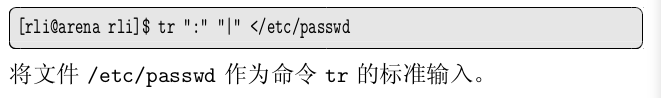
\includegraphics[scale=0.6]{./figures/231.png}
%%\caption{}
\end{figure}

$\bullet$~重定向标准输出
\begin{figure}[H]
\centering
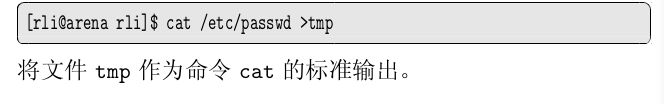
\includegraphics[scale=0.6]{./figures/232.png}
%%\caption{}
\end{figure}
$\bullet$~重定向标准错误
\begin{figure}[H]
\centering
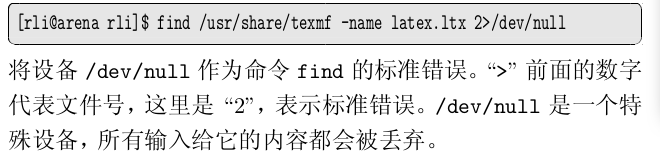
\includegraphics[scale=0.6]{./figures/233.png}
%%\caption{}
\end{figure}
$\bullet$~同时重定向标准输入、标准输出和标准错误
\begin{figure}[H]
\centering
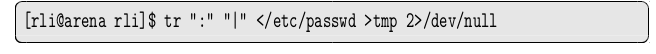
\includegraphics[scale=0.6]{./figures/234.png}
%%\caption{}
\end{figure}
$\bullet$~将标准错误定向到标准输出
\begin{figure}[H]
\centering

\includegraphics[scale=0.6]{./figures/235.png}
%%\caption{}
\end{figure}
该例中,首先将标准输出定向到文件 tmp ,再将标准错误定向到标准输出。注意, “2>\&1” 的含义是将标准错误 (2) 定向到标
准输出 (1) 当前所关联的文件或设备,因此, “>tmp 2>\&1” 与“2>\&1 >tmp” 的结果是不同的,前者中标准错误被定向到文件tmp ,而后者中标准错误被定向到终端,因为当遇到 “2>\&1” 时标准输出依然是终端!

当用 “>” 将标准输出或标准错误重定向到一个文件时,如果指定的文件不存在,则会建立一个新文件;如果文件已经存在,那么,该文件的内容会首先被清空。如果想保留文件的原有内容,而将输出添加在文件的最后,可以用连续两个大于号 “>>” 代替 “>” 。

对于标准输入,也可以用连续两个 “<” ,即 “<<” ,来进行重定
向。看下面的例子:
\begin{figure}[H]
\centering
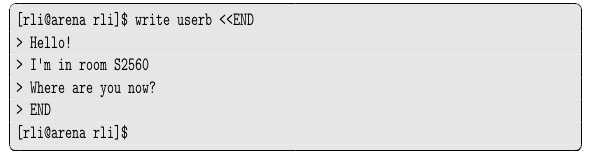
\includegraphics[scale=0.6]{./figures/290.png}
%%\caption{}
\end{figure}

注意 “<<” 后面跟随的不是一个文件名或设备名,而是一个用于标志标准输入结束的字符串。如果在一个 shell 脚本中使用 “<<” ,则脚本中的后续内容会被作为标准输入的内容,直到遇到标志结束的字符

管道在 shell 中,它指用符号 “|”将一个命令和另一个命令连接起来,将前一个命令的标准输出作为后一个命令的标准输入,下面的例子通过一串管道操作,取出本机器的 IP 地址。用命令 /sbin/ifconfig 可以得到关于网卡的信息,例如
\begin{figure}[H]
\centering
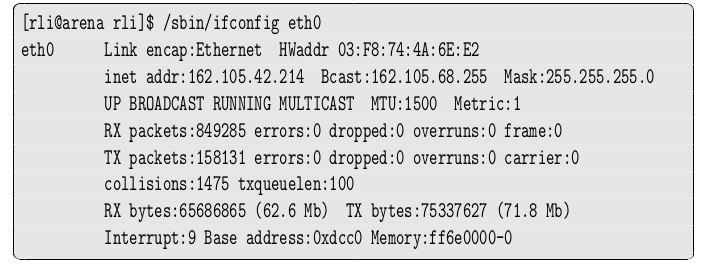
\includegraphics[scale=0.6]{./figures/236.png}
%%\caption{}
\end{figure}
利用管道,对上面的输出进行进一步处理,可以将想要的信息 (IP 地
址 ) 提取出来:
\begin{figure}[H]
\centering
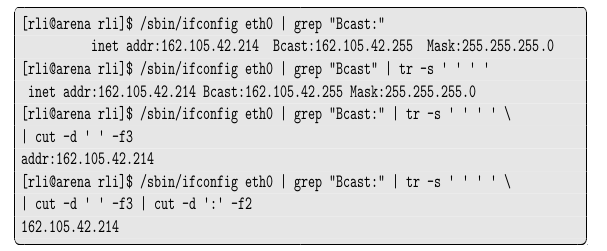
\includegraphics[scale=0.6]{./figures/277.png}
%%\caption{}
\end{figure}
可以看到机器的 IP 地址在 ifconfig 命令的输出的第二行,该行中包含有一个特有的词 “Bcast:” 。因此,首先用 grep 查找关键词 “Bcast:” 将第二行单独提取出来。然后,用 tr 命令将连续多个空格合并成为一个空格,再用空格作为分隔符将该行内容分成
四列,用 cut 命令取出第三列得到字符串 “addr:162.105.42.214” 。最后,用 “:” 作为分隔符取出第二列,便是机器的 IP 地址。该例中通过管道,用不同命令反复对输出进行处理,提取出最终的信息。这是 shell 中处理文本最常用的办法。

\textbf{5.环境变量}

Linux 系统启动的时候,会启动一个特殊的进程,名为 init ,它负责控制整个系统的运行及启动所有其他进程。当用户登录进入系统的时候,首先得到一个 shell ,它也是一个进程,其中中执行的命令都是该 shell 的子进程。事实上,只有当获得一个 shell 后,用户才真正开始和计算机沟通,例如输入命令、执行程序等等。在一个 shell中,可以再进入另外一个 shell ,即启动一个子 shell ,然后还可以再进入更深一层的 shell 。每次输入 exit 命令则退出一层 shell ,回到上一个 shell 中。任何一个进程都可以启动其他一些进程,这些进程称为该进程的子进程,而该进程则被称为这些进程的父进程。在实际应用中,往往需要从父进程向子进程传递一些初始参数或设置。通常,有两个方法从父进程向子进程传递初始参数,第一个方法是在启动子进程时通过命令行参数传递,第二个方法是通过环境变量传递。

在 Linux 的进程中,变量是一个具有自己的名字,其值能够在一定范围内保持和被改变的量。当启动一个子进程时,父进程中定义的部分变量会被子进程所继承。由于这些变量起着设定进程的运行环境的作用,因而被称为环境变量(environment variables) 。

环境变量名称通常用大写字母表示。 Linux 只负责在进程间传递环境变量的值,至于如何使用这些环境变量是由进程自行决定的。但是,有一组环境变量的作用是所有进程共同遵循的,这里称它们为标准环境变量。下表列出了一些常用的标准环境变量,以及Bash 中常用的一些环境变量。
\begin{figure}[H]
\centering
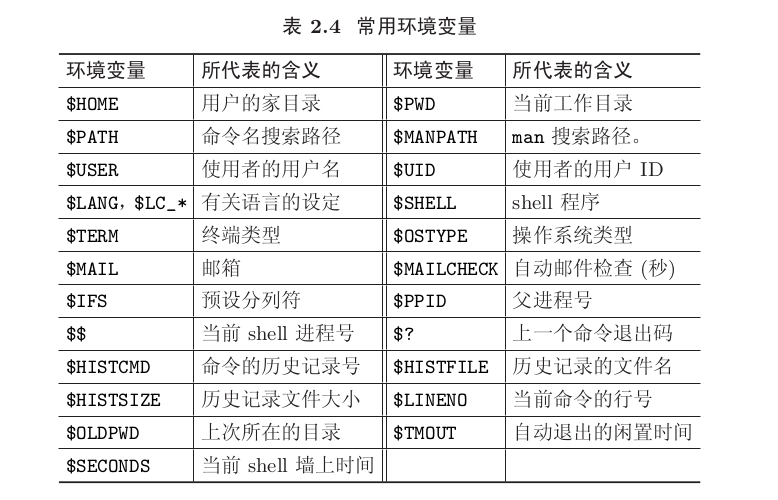
\includegraphics[scale=0.6]{./figures/273.png}
%%\caption{}
\end{figure}
在 shell 中,如果想引用某个环境变量的值,只要在变量名称前面加上一个 “\$” 。例如
\begin{figure}[H]
\centering
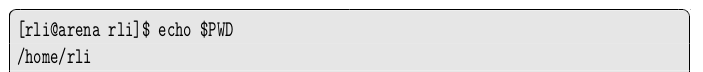
\includegraphics[scale=0.6]{./figures/238.png}
%%\caption{}
\end{figure}
如果想定义一个新的环境变量,或者改变现有环境变量的值,用
等号 “=” 就可以了。例如:
\begin{figure}[H]
\centering
\includegraphics[scale=0.6]{./figures/239.png}
%%\caption{}
\end{figure}
想要删除一个环境变量,可以用 unset 命令:
\begin{figure}[H]
\centering
\includegraphics[scale=0.6]{./figures/240.png}
%%\caption{}
\end{figure}

在 shell 中,新定义的环境变量默认是不传递给 shell 的子进程的。如果想将新定义的环境变量传递给子进程,必须用 export 命令输出该变量。作为一个子进程,它只继承自己启动时父进程所传递的环境变量。子进程开始运行后是无法得到父进程新定义的环境变量、或是修改的环境变量值的。反过来,子进程对环境变量的改变对父进程没有影响。请看下面的例子:
\begin{figure}[H]
\centering
\includegraphics[scale=0.6]{./figures/241.png}
%%\caption{}
\end{figure}
在定义环境变量时还需要注意一些细节:

$\bullet$~ 定义环境变量时, “=” 号两边不能有空格;

$\bullet$~ 环境变量的名称,只能是字母、数字和下划线,且不能以数字开
头;

$\bullet$~ 系统预定义的环境变量均为大写;

$\bullet$~ 如果环境变量的值中带有特殊字符或空格,必须用 “$\setminus$” 转义,
或用引号将环境变量的值引起来;

shell 中引号的作用,括在单引号 “'” 中的内容,所有字符都作为普通字符处理,任何特殊字符,除单引号外,都失去其特殊含义。但单引号中不能再使用单引号。而在双引号中,某些特殊字符,如 “\$” 、 “$\setminus$” 等,依然保留其特殊的功能。

除了可以用外部命令,如 grep 、 cut 等,处理环境变量中的字符串, Bash 本身也提供了一些对环境变量的值进行过滤、处理的功能。 Bash 中常用的过滤语法和规则在下表中给出。在这些过滤规则中,字符 “*” 用于匹配任意字符串。
\begin{figure}[H]
\centering
\includegraphics[scale=0.6]{./figures/242.png}
%%\caption{}
\end{figure}

\textbf{6. 命令行展开}在Linux bash中可以使用命令行展开特性一步完成需要分开成多步完成的操作,达到事半功倍的效果。

$\bullet$~ 花括号展开:在Linux指令参数位置使用"{}" 将相应的参数括起来,括号中的参数以逗号分隔,然后bash在执行这一指令时会自动将括号中的内容进行展开。同时创建多个目录,在/test1目录下创建ac,ad,bc,bd:
\begin{figure}[H]
\centering
\includegraphics[scale=0.6]{./figures/244.png}
%%\caption{}
\end{figure}
$\bullet$~ 波浪号 (~) 展开:一个单独的 “~” 展开为当前用户的家目录,即环境变量 \$HOME 的值,而 “~用户名” 则展开为此用户的家目录;

$\bullet$~ 变量展开:一个变量名前面加上一个 “\$” ,就会进行变量展开,展开的结果就是这个变量的值。

$\bullet$~ 命令替换:命令替换指用一个命令执行的结果来替换这个命令本身。命令替换可以用两个方式实现: “\$( 命令 )” 或者 “ \` 命令 \` ”
\begin{figure}[H]
\centering
\includegraphics[scale=0.6]{./figures/294.png}
%%\caption{}
\end{figure}
由上可知:反引号中\$并没有将\$的特殊意义转换 ,反引号包含的内容 echo \$HOSTNAME 仍然被解释为一个echo,$\setminus$HOSTNAME 取到了这个变量的值并输出。

()则正好相反,\$明显被$\setminus$转义成了一个普通字符,所以并没有取到变量值,而是返回了字符串本身的意思,故而返回了HOSTNAME。

$\bullet$~ 算术展开:算术展开的形式为 “\$(( 算术表达式 ))” 。表达式中的所有部分会首先进行参数展开、命令展开和引号去除,然后再进行算术运算,运算结果便是展开结果。

$\bullet$~ 参数分割:将上面的各种展开后的结果分解为分离的一个一个词。双引号或单引号的内容不会被分开,如下:
\begin{figure}[H]
\centering
\includegraphics[scale=0.6]{./figures/295.png}
%%\caption{}
\end{figure}

$\bullet$~ 文件名展开:在参数分割以后,如果命令中没有 “-f” 选项, Bash会扫描每个词,在里面寻找 “*” 、 “?” 和 “[” 这三个字符。如果找到了,那么这个词就被作为一个模板,替换成一串与其相匹配的文件名。这些文件名按照字母顺序排列。如果没有任何与之相匹配的文件,而 Bash 选项 “nullglob” 又被禁止的话,那么这个词将会原封不动地保留下来;如果没有禁止 Bash 选项
“nullglob” ,而又没有匹配到任何文件,那么这个词就会被去掉。如果设置了 Bash 选项 “nocaseglob” ,那么在进行匹配的时候将忽略字母大小写的不同。

当对一个模板进行文件名展开时,如果没有设置 Bash 选项“dotglob” ,则当字符 “.” 出现在一个文件名的开头或者在一个斜杠之前时必须精确地和 “.” 匹配,即不包含在 “?” 或 “*” 中。斜杠 “/” 总是被精确匹配。其他情况下,字符 “.” 与其他字符一样,可以被 “?” 或 “*” 匹配。

进行模板匹配的规则如下:如果不是下面列举的特殊字符,那么字符将和它自己相匹配。在模板中,不能出现 NUL (ASCII0)字符。如果想匹配特殊字符,可以用引号将它们引起来。模板中的特殊字符及含义如下:

– “*” :和任何字符串相匹配,包括空字符串;

– “?” :和任何单个字符相匹配;

– “[...]” :和方括号中指定的任何一个字符相匹配。


$\bullet$~ 引号去除:在完成前面所有这些展开以后,所有没有被引起来的反斜杠、单引号和双引号,如果不是前面这些展开的结果、而是最初的输入话,会全部被扔掉。

\textbf{Shell 脚本}

shell 使用方法有交互式的 (Interactive) shell ,Shell 也有以非交互的方式运行,类似于 MSDOS 中的批命令文件。即将一大段 shell 命令放在一个文件中,然后让 shell 以批处理的方式执行所有命令。这样的文件叫做 shell 脚本(shell script) 。

Bash 读入、执行一条命令的过程可分解为下面七个步骤:

(1) 从文件或者用户的终端读入字符串;

(2) 将输入分解成为“词”和“操作符”。在这一步中,会对引号进行处理,进行 alias 替换;

(3) 将这些“词”和“操作符”分解成简单命令或者组合命令;

(4) 进行各种各样的 shell 展开,将展开结果分解成命令名、文件名、参数等;

(5) 进行输入输出重定向并将重定向符号和重定向参数从参数表中去掉;

(6) 执行上面一系列处理后得到的最终命令;

(7) 等待命令执行完成并得到命令执行的结果 ( 返回码 ) ;如果将命令放到后台执行,则 Bash 将不等待命令的完成而直接转入处理下一条命令。

下面比较详细地介绍一下 Bash 作为一种程序语言的语法。首先介绍 Bash 的词法和保留词。 Bash 将一行命令分解成为一个个单独的“词”,分隔这些词的字符包括下面一些:
\begin{figure}[H]
\centering
\includegraphics[scale=0.6]{./figures/245.png}
%%\caption{}
\end{figure}
其中空格和制表符的作用是一样的,它们都被称为“空白”。这些词中有两类比较特殊。一类是“标识符”,由字母、数字和下划线组成,而且开头不能是数字。另一类是“控制符”,控制符只有下面几个:
\begin{figure}[H]
\centering
\includegraphics[scale=0.6]{./figures/246.png}
%%\caption{}
\end{figure}
有一组词对于 Bash 来说有特殊的含义,它们叫做保留词。当这些词没有被引号引起来的时候会起到特殊的作用。这些保留词有:
\begin{figure}[H]
\centering
\includegraphics[scale=0.6]{./figures/247.png}
%%\caption{}
\end{figure}
Bash 的语法基本上可以用下面几条来描述:

$\bullet$~ 单个命令 (simple command) :单个命令包括一个命令名、用空格分开的参数、重定向操作符和一个控制符结尾。简单命令的返回值是所执行的命令的退出码。如果命令执行时被一个信号终止,那么返回值是 128 加上信号值。

$\bullet$~ 流水线 (pipeline) :流水线指一系列用管道连接起来的命令。由于管道具有比重定向更高的优先级别,因此如果同时使用了管道和重定向,输出内容将被定向到管道中。流水线的语法是
\begin{figure}[H]
\centering
\includegraphics[scale=0.6]{./figures/248.png}
%%\caption{}
\end{figure}
整个命令的返回值是最后一条命令的返回值。如果加了感叹号
“!” ,则返回值是最后一条命令的返回值的“逻辑否”。如果前面加了关键字 “time” ,则命令结束时 Bash 会报告执行命令所花费的时间,包括墙上时间和 CPU 时间。如果在 time 后面使用了选项 “-p” ,则输出运行时间时将采用 POSIX 格式。

$\bullet$~ 命令序列 (list) :一个命令序列就是用下面的符号连接起来的一串单个命令或流水线:
\begin{figure}[H]
\centering
\includegraphics[scale=0.6]{./figures/249.png}
%%\caption{}
\end{figure}
这些命令的最后必须用 “;” 、 “$\&$” 或者换行结束。用 “$\&$” 结束表示将命令放到后台去执行。后台执行的命令实际上是在一个子shell 中执行,此时命令序列的返回值是 0 。对于其他情形,命令序列的返回值为最后一条命令的返回值。用 “;” 连接起来的命令按照顺序依次执行, Bash 会一直等
待它们全部执行完。“$\&\&$” 和 “||” 的作用类似于 C 语言中的同名逻辑运算符,前者表示“与”,后者表示“或”,操作对象是命令的返回值,返回值为 0 表示“真”,返回值非 0 则表示“假”,采用短路规则。它们的语法分别是
\begin{figure}[H]
\centering
\includegraphics[scale=0.6]{./figures/250.png}
%%\caption{}
\end{figure}
\begin{figure}[H]
\centering
\includegraphics[scale=0.6]{./figures/251.png}
%%\caption{}
\end{figure}
对第一种情况,当命令 1 的返回值为 0 ( “真” ) 时命令 2 才执行;而对于第二种情况,当命令 1 的返回值是非 0 ( “假” ) 时命令 2
才会执行。两种情况中命令序列的返回值都是最后所执行的命令的返回值。

$\bullet$~条件判断:

\begin{figure}[H]
\centering
\includegraphics[scale=0.6]{./figures/278.png}
%%\caption{}
\end{figure}
其中方括号表示可以省略的部分。

$\bullet$~ 循环语句:循环语句有 4 种形式。第一种形式为:
\begin{figure}[H]
\centering
\includegraphics[scale=0.6]{./figures/254.png}
%%\caption{}
\end{figure}
第二种循环形式为:
\begin{figure}[H]
\centering
\includegraphics[scale=0.6]{./figures/255.png}
%%\caption{}
\end{figure}
其他两种循环形式分别为:
\begin{figure}[H]
\centering
\includegraphics[scale=0.6]{./figures/256.png}
%%\caption{}
\end{figure}
这些循环的用法可用下面四个例子说明,它们完成同样的工作:
\begin{figure}[H]
\centering
\includegraphics[scale=0.6]{./figures/257.png}
%%\caption{}
\end{figure}
最后,还有一种选择形式的复合命令,句法如下:
\begin{figure}[H]
\centering
\includegraphics[scale=0.6]{./figures/258.png}
%%\caption{}
\end{figure}
其含义是执行与 “ 词 ” 相匹配的第一个模版后面的命令。在模版中可以用 “*” 匹配任意子串,用 “|” 表示“或”运算,如“abc*|def*)” 表示匹配以 “abc” 或 “def” 开头的字符串。如果模版由单独一个 “*” 构成,则表示它与任意字符串相匹配,通常放在最后用来定义默认处理。选择命令的例子如下:
\begin{figure}[H]
\centering
\includegraphics[scale=0.6]{./figures/259.png}
%%\caption{}
\end{figure}
脚本文件的第一行通常是下面的形式:
\begin{figure}[H]
\centering
\includegraphics[scale=0.6]{./figures/260.png}
%%\caption{}
\end{figure}
这里, \#! 后面的文件的名叫做命令解释器 (command interpreter) 。

下面是 shell 脚本的基本结构:

$\bullet$~ 简单说来,一个 shell 脚本就是一连串命令行,再加上一些条件
判断、循环、跳转等语句;

$\bullet$~ 每当 shell 解释器在脚本中读到一个回车符的时候,就尝试执行
该行命令;

$\bullet$~ Shell 解释器会忽略空白行,以及一行开头的空白和 <Tab> ;

$\bullet$~ 回车符同样可以用 “$\setminus$” 符号进行转义,转义后的回车符相当于
一个空白,通常用来表示连续行,即将下一行的内容和这一行
合并起来当作一行处理;

$\bullet$~ “\#” 是注释符号,从它开始至当前行尾的内容都是注释。利用注
释符号,可以在脚本中插入一些注解。

有两个方法执行一个 shell 脚本,一个方法是将文件名作为bash 命令的参数,此时 Bash 会忽略脚本文件第一行 “\#!” 后面指定的解释器。另外一个方法是直接将脚本文件名作为命令名执行。要想直接执行一个 shell 脚本文件,用户必须对它有执行权限。用文件编辑器新建立的文件一般都是没有执行权限的,需要用 chmod 命令加上。


Bash 有一条内部命令 “test” ,能够对一些条件进行检测。例
如: “test -f \~/src/rli.cpp.bak” 检测文件 \~/src/rli.cpp.bak
是否存在并且是否是一个普通文件,若文件存在则返回 0 ,否则返回
1 。除了 “-f” 外, test 还支持很多测试选项,见表 2.6 ,它们在 shell
脚本中非常有用。 test 命令通常用在 if 语句中,根据检测的结果
控制脚本的执行流程。
\begin{figure}[H]
\centering
\includegraphics[scale=0.6]{./figures/261.png}
%%\caption{}
\end{figure}
除了对单个文件进行检测外, test 命令也可以用来比较两个文件。例如: “test 文件 1 -nt 文件 2” 检测文件 1 是否比文件 2 新。这些检测使用的比较操作符在下表中给出。
\begin{figure}[H]
\centering
\includegraphics[scale=0.6]{./figures/262.png}
%\caption{}
\end{figure}

除了检测文件外, test 命令也可以进行算术比较和字符串检测。用于算术比较和字符串检测的操作符列由下表给出。事实上,可以检测的项目还有很多,用 man test 和 man bash 可以得到详尽的说明。
\begin{figure}[H]
\centering
\includegraphics[scale=0.6]{./figures/275.png}
%\caption{}
\end{figure}
Shell 的变量可以作为算术表达式中的操作数。在求值以前,会优先进行参数展开。还有一点要指出的是,在 “\$(( ... ))” 的表达式中引用 shell 变量时可以省略变量前
面的 “\$” ,例如:
\begin{figure}[H]
\centering
\includegraphics[scale=0.6]{./figures/276.png}
%\caption{}
\end{figure}
如果想在 shell 中进行浮点数运算,可以借助于外部程序 bc 来进行,例如:

\begin{figure}[H]
\centering
\includegraphics[scale=0.6]{./figures/263.png}
%\caption{}
\end{figure}

\begin{figure}[H]
\centering
\includegraphics[scale=0.6]{./figures/264.png}
%\caption{}
\end{figure}


\textbf{8. 命令行参数}

当运行一个 Bash 脚本或函数 ( 关于 shell 函数的的说明参看下节 ) 的时候,命令行上脚本或函数名后面给出的参数会被传递给脚本程序或函数。 Bash 根据分隔字符 ( 由环境变量 IFS 定义,通常是空格 ) 将参数分割成一个个的词,每个词作为一个参数,从 1 开始编号。如此分割后的参数称为位置参数。如果一个参数本身包含分隔字符,但又不希望 Bash 将其当作两个参数处理,可以在命令行上用双引号或单引号将它括起来,或是用 “$\setminus$” 对分隔字符进行转义。 Bash 脚本中用 “\$1” 、 “\$2” 等引用位置参数,其中 “\$1” 表示第一个参数, “\$2” 表示第二个参数,依此类推。引用一个不存在的参数得到的是空字符串。此外, “\$0” 表示 Bash 脚本本身的文件名, “\$\#”表示位置参数的个数, “\$\*” 或 “\$@” 表示所有位置参数 (list) 。作为一个特例, “"\$@"” ( 注意这里的双引号 ) 也表示全部位置参数,它被展开后,每个参数会括在一对双引号中,可用于处理参数中包含分
隔字符的情形。命令 “shift [n]” 对位置参数进行“平移”操作,表示删除前 n 个位置参数,省略 n 时删除第一个位置参数。位置参数除了可以从命令行获得外,也可以用 Bash 的内部命
令 “set” 来指定或改变,这里不做介绍。

\textbf{9. Shell 函数}

Bash 允许用户定义函数。一个函数一旦定义,可以像其他内部
或外部命令一样使用。 Bash 的函数定义采用下面形式:
\begin{figure}[H]
\centering
\includegraphics[scale=0.6]{./figures/279.png}
%\caption{}
\end{figure}
Bash 函数中也可以使用位置参数,它们就是调用函数时给出的参数。函数中用 “return [ 返回码 ]” 返回,其中 “ 返回码 ” 的含义和其他命令的返回码是一样的, 0 表示成功。在 Bash 函数中,还可以用local 命令声明局部变量。
\subsubsection{文本文件处理}
\textbf{1. 正则表达式}

正则表达式是一种特殊格式的模版,能够和其他字符串进行灵活的匹配,从而迅速完成一些复杂的文本处理工作。这里先给出正则表达式的语法及匹配规则。在 Linux 中,可以用 “man 7 regex” 得到 POSIX 1003.2正则表达式语法的在线文档。
一些软件,包括一些
版本的 sed 、 vi 、 awk 等,依然使用老的正则表达式格式,它们将
“+” 、 “(” 、 “)” 、 “|” 等当作普通字符处理,必须在它们前面加上 “$\setminus$”
才具有下面介绍的元字符的功能 ( 例如,需要将正则表达式 “(a|b)+”
写成 “$\setminus$(a$\setminus$|b$\setminus$)$\setminus$+” 的形式 ) 。

一个正则表达式就是一个字符串。字符串中的字符分成两类,一类是普通字符,另外一类是特殊字符,叫做元字符,元字符有下面一些:
\begin{figure}[H]
\centering
\includegraphics[scale=0.6]{./figures/280.png}
%\caption{}
\end{figure}
这些元字符的基本涵义如下:

$\bullet$~“*” :作为后缀使用,表示将其前面匹配的字符串连续地重复 0
次到任意多次。比如 “o*” 会匹配一连串任意多个 “o” ( 包括空
字符串 ) 。要注意的是,它只是对前面的最小匹配进行重复,比
如 “fo*” 会匹配 “f” 后面紧跟着零个或者任意多个 “o” 的情
况,而不是零个或者任意多个 “fo” 。用 “*” 进行匹配时,会首
先尽量匹配多的内容,直到不能匹配为止,然后,会根据跟随其
后的表达式的匹配需要,回吐一部分已经匹配的内容;

$\bullet$~ “+” :和 “*” 的含义相近,但要求前面的表达式至少匹配上一次。
例如 “ca+r” 会与 “car” , “caaaar” 匹配,但是却不会与 “cr”
匹配;

$\bullet$~ “?” :将前面的表达式匹配一次或零次。例如, “ca?r” 只与 “car”
或 “cr” 匹配;

$\bullet$~ “\{n\}’ :这里 n 代表一个整数,表示将前面匹配的内容连续匹配
n 次。例如, “x{4}” 与 “xxxx” 匹配;

$\bullet$~ “\{n,m\}” :表示将前面的内容连续至少匹配 n 次,至多匹配 m
次。省略 m 时表示 m 为无穷。容易看出, “\{0,1\}” 和 “?” 是等
价的, “\{0,\}” 和 “*” 是等价的,而 “\{1,\}” 和 “+” 是等价的;

$\bullet$~ “[...]” :表示一个字符集,由一个左方括号开始,一个右方括
号结束,中间列出字符集中的字符。

$\bullet$~ “[$~\hat{}~$ ... ]” :匹配的字符集为方括号中的字符集的补集,即与
任何不属于方括号中的字符集的字符匹配。

$\bullet$~ “$~\hat{}~$” :如果不在方括号中,则表示一个行的行首,也就是说,紧跟在其后的表达式必须匹配一行开头的字符串;

$\bullet$~ “\$” :和 “$~\hat{}~$”相对应,表示一行的结尾;

$\bullet$~ “$\setminus$” :用于将元字符进行转义。比如想匹配一个 “[” 的话必须使
用 “$\setminus$ [” ,想匹配一个 “\$” 的话必须使用 “$\setminus$\$” ;

$\bullet$~ “|” :表示“或”的意思,用它将一组正则表达式连接起来构成一
个新的正则表达式,一个字符串只要与这些正则表达式中的任
何一个匹配,便与整个正则表达式匹配。例如,表达式 “ab|cd”
同时匹配 “ab” 和 “cd” ;

$\bullet$~ “(...)” :其中括号中是一个正则表达式。圆括号在正则表达式
中的作用与普通表达式中类似,用来将一组正则表达式组合在
一起,当作一个整体看待。


\textbf{2. sed 和 awk}

sed 是所谓的流编辑器 (stream editor) 。它所完成的工作就是
对一个输入的文本流进行一定的转换,就象是对文件进行了编辑一
样。sed 和其他编辑器的一个重要不同之处在于它能够在管道上进
行操作,是非交互式的,处理的效率很高。

sed 在工作时接受一个输入流,并同时需要获得对流进行操作
的命令脚本。输入流可以通过管道、命令行上的文件名、重定向或者
是一个字符串等方式获得,而命令脚本是通过命令行的 -e 或者 -f
选项获得的。如果是 -e 选项,那么后面紧跟的字符串就是脚本,如果是 -f 选项,那么后面是一个文件名,该文件中的文本就是命令脚
本。记录着 sed 命令的脚本文件叫做 sed 程序, sed 程序中的内容
是一条一条的 sed 命令。 sed 从输入流中读取一段数据,存储在缓
冲区中,然后依次使用命令脚本中的每条命令对缓冲区中的内容进
行处理,最后将得到的结果输出到标准输出。通过重定向,可以将
sed 运行的结果保存到文件中。

下面看一个简单的例子:
\begin{figure}[H]
\centering
\includegraphics[scale=0.6]{./figures/281.png}
%\caption{}
\end{figure}
这里 -e 选项后面紧跟的就是命令脚本。这条命令的意思是这样的:
对于文本中从第 20 行到最后一行进行替换操作,将和正则表达式
“ca*r” 匹配的字符串的第一个字符 “c” 替换为 “b” ,最后一个字符
“r” 替换为 “t” ,中间部分保持不变。使用 “$\setminus$(” 和 “$\setminus$)” 括起来的
部分被赋予了一个名字叫做 “$\setminus$1” ,可以在替换的字符串中对其进行
引用。如果正则表达式中有多个这样的部分,则分别用 “$\setminus$1” , “$\setminus$2”
等表示。这条命令由下面几部分
构成:首先指定操作的范围,这里是 “20,\$” ,表示从第二十行到最
后一行;然后是命令 “s” ,表示进行替换,它是 sed 中最常用的命
令,其他命令还有删除 (d) 、打印 (p) 等,由于不常用到,这里不做
介绍;接着给出被替换的字符串 ( 正则表达式 ) 和替换的结果;最后
的 “g” 是一个操作标识,意为 global ,表示替换所有匹配的字符串
( 没有 “g” 时只替换每行中第一个匹配的字符串 ) ,其他的标识请参
考 sed 的在线文档。 “s” 命令的一般形式为:
\begin{figure}[H]
\centering
\includegraphics[scale=0.6]{./figures/282.png}
%\caption{}
\end{figure}
其中方括号表示可以省略的部分 ( 即“范围描述”和“操作标识”,省
略前者时表示操作范围为所有行 ) 。

awk 是一种解释性的编程语言,其语法
是比较复杂的,当然功能也非常强大。它的基本工作方式和 sed 相
近,对一个流进行扫描,遇到特定的字符串时执行特定的操作,但是
它的功能比 sed 要丰富得多。和 sed 一样, awk 在运行的时候,需
要获得两个输入信息,一个是要处理的流,另外一个是匹配规则与
处理命令。要处理的流可以是标准输入,也可以是用命令行参数指
定的文件。处理命令可以直接在命令行中给出,也可以写在一个脚
本文件中。awk 的处理命令的格式为:
\begin{figure}[H]
\centering
\includegraphics[scale=0.6]{./figures/283.png}
%\caption{}
\end{figure}
其中处理方法部分的语法和 C 语言的语法类似,但是 awk 有自己的
一套函数,可以参考 awk 的在线文档了解有关这些函数的细节。除
了函数之外, awk 还有一些预定义的基本变量,在进行字符串处理时
经常用到。 awk 处理时假设文本是分列的,它用变量 “\$n” , n 是一
个整数,表示第 n 列, \$0 表示整个行。



\textbf{3. diff 和 patch}

diff 用来将两个文件的不同之处找出来,它的基本工作方式是按行进行操作的,所以一般用于文本文件。其命令的基本形式为
\begin{figure}[H]
\centering
\includegraphics[scale=0.6]{./figures/270.png}
%\caption{}
\end{figure}

patch 就是打补丁的
意思。例如,用户从网上下载了一个比较大的软件,后来该软件有一
个比较小的修改,此时当然希望仅仅下载修改的部分,而不用重新
下载整个软件。软件作者通常会提供用 diff 命令得到的补丁文件,
只要下载补丁文件,然后用命令 patch 就可以自动更新原先下载的
软件。 patch 的命令行形式有两种,第一种是:
\begin{figure}[H]
\centering
\includegraphics[scale=0.6]{./figures/271.png}
%\caption{}
\end{figure}
其中 “ 补丁文件 ” 便是 diff 命令产生的输出。对于从网上下载的软
件补丁,经常使用的是第二种形式:

\begin{figure}[H]
\centering
\includegraphics[scale=0.6]{./figures/272.png}
%\caption{}
\end{figure}
它可以自动更新整个目录中修改过的文件。其中选项 “-p 数字 ” 表
示寻找要修改的文件时去掉补丁文件中指定的路径名开头的几层目
录, “ 数字 ” 是一个整数,用来指定要去除的目录层数。运行 patch
后,目录中的相关文件就会变成更新后的版本。

利用 diff 和 patch 可以对文本文件进行非常灵活的操作,对
于文本文件的修改、维护及协同操作非常有用。

\cite{tam19912d}

%\bibliography{../ref}
\end{document}
